% This is samplepaper.tex, a sample chapter demonstrating the
% LLNCS macro package for Springer Computer Science proceedings;
% Version 2.20 of 2017/10/04
%
\documentclass[runningheads]{llncs}
%
\usepackage{graphicx}
\usepackage{amssymb}
\usepackage{amsmath}
\usepackage{hyperref}
\usepackage{tikz}
\usetikzlibrary{matrix}
\usepackage[toc,page]{appendix}

% Used for displaying a sample figure. If possible, figure files should
% be included in EPS format.
%
% If you use the hyperref package, please uncomment the following line
% to display URLs in blue roman font according to Springer's eBook style:
% \renewcommand\UrlFont{\color{blue}\rmfamily}

\begin{document}
%
\title{An Evaluation of Uninformed and Informed Search Algorithms on the k-puzzle Problem\thanks{Supported by Prof Yair Zick and Prof Daren Ler.}}
%
\titlerunning{Evaluation of Search Algos on k-puzzle}
% If the paper title is too long for the running head, you can set
% an abbreviated paper title here
%
\author{Dalis Chan \textit{(A0187451Y)} \and
Johanna \textit{(A0187536R)} \and
Sean Low Chen Yi \textit{(A0183743Y)} \and 
Law Ann Liat, Larry \textit{(A0189883A)}}
%
% First names are abbreviated in the running head.
% If there are more than two authors, 'et al.' is used.
%

\institute{National University of Singapore \\
Repository Link \href{https://github.com/larrylawl/CS3243-project-1}{here}}
%
\maketitle              % typeset the header of the contribution
%
\begin{abstract}
K-puzzle is often used as test problems for new search algorithms in artificial intelligence ~\cite[p71]{stuart_russell_artifical_2010}. This paper evaluates the use of iterative deepening search (IDS) and \( A^* \) search. 
Since \( A^* \) search uses heuristic functions to guide its search, this paper also evalutes the heuristic functions euclidean distance, manhattan distance, and linear conflict.
\end{abstract}
%
%
%
\section{Problem Specification}
\begin{enumerate}
    \item \textbf{State:} For \( k \in \{3, 4, 5\} \),  a \( k \times k \) matrix \( M \) with each entry \( m_{i, j} \) being a unique integer from \( \{0, 1, \cdots, 8 \} \) where 0 represents the blank tile.
    \item \textbf{Initial State:} Puzzle can start in any state \textit{s}.
    \item \textbf{Actions or \textit{Actions(s)}:} Let \( m_{k, l} \in M \) denote the blank tile and \( m_{i, j} \in M \) denote the tile \textbf{adjacent} to the blank tile \( m_{k, l} \).
    Actions are movements of the adjacent tile \( m_{i, j} \) towards the blank tile \( m_{k, l} \). For example, the action \textit{Left} moves the adjacent tile \( m_{k, l+1} \in M \) to the blank tile \( m_{k, l} \).
    \item \textbf{Transition Model or \textit{Result(s,a)}:} \( Result(s, a) \) swaps the pair of tiles specified in action \( a \) in the current state \textit{s} and returns this new state \textit{s'}.
    \item \textbf{Goal State:} 
    \[
    M_{goal}= \begin{bmatrix}
        1 & 2 & \cdots & k \\
        k+1 & k+2 & \cdots & 2k \\
        \vdots & \vdots & \vdots \\
        k^2 - k + 1 & k^2 - k & \cdots & 0
        \end{bmatrix}
    \]
    \item \textbf{Path Cost:} Every step cost \textit{c(s, a, s') = 1}, and the path cost is the summation of the step costs from the initial state to the goal state.
\end{enumerate}

\section{Technical Analysis of the Selected Algorithms and Heuristics}
\label{section2}

\subsection{Rule to Check if k-puzzle is Solvable}
\textbf{Definition.}~\cite{aditya_goel_how_nodate}. A pair of tiles form an \textit{inversion} if the values on tiles are in the reverse order of their appearance in the goal state. \\
\textbf{Rules}~\cite{aditya_goel_how_nodate}. Let \( M \) denote a \( k \times k \) matrix, \( m_{i, j} \) denote a blank tile in \( M \), and \( n_i \) denote the number of inversions in the intial state \( M_{initial} \). Puzzle is solvable if \dots
\begin{enumerate}
    \item \( k \) is odd and \( n_i \) is even
    \item \( k \) is even,
    \begin{enumerate}
        \item \( n_i \) is odd and \( m_{i,j} \) is on an even row from the bottom (ie \( j \) is odd).
        \item \( n_i \) is even and \( m_{i,j} \) is on an odd row from the bottom (ie \( j \) is even).
    \end{enumerate}
\end{enumerate}

\subsection{Uninformed Search}
\begin{enumerate}
    \item \textbf{Implementation:} Graph-based IDS. Step costs are equal, thus it is optimal~\cite[p88]{stuart_russell_artifical_2010}. Furthermore, since the search space is large and the depth of the solution is not known, IDS is preferred ~\cite[p90]{stuart_russell_artifical_2010}.
    \item \textbf{Correctness:} Branching factor \( b = 4 \) is finite, thus IDS is complete ~\cite[p88-90]{stuart_russell_artifical_2010}. 
    \item \textbf{Time Complexity:} \( O(b^d) \) ~\cite[p88-90]{stuart_russell_artifical_2010}.
    \item \textbf{Space Complexity:} \( O(bd) \) ~\cite[p88-90]{stuart_russell_artifical_2010}.
\end{enumerate}

% TODO Add in proofs for heuristic
\subsection{Informed Search}
\begin{enumerate}
    \item \textbf{Implementation:} Graph-based \( A^* \) search. It improves on greedy best first search (ie \( f(n) = h(n) \)) as it avoids expanding paths that are already expensive (ie \( f(n) = g(n) + h(n) \)).
    \item \textbf{Correctness:} Since the search space is finite, \( A^* \) search will be complete.
    \item \textbf{Time Complexity:} \( O(b^{h^*(s_0) - h(s_0)}) \) ~\cite[p93-99]{stuart_russell_artifical_2010}.
    \item \textbf{Space Complexity:} \( O(b^m) \) ~\cite[p93-99]{stuart_russell_artifical_2010}.
\end{enumerate}

\subsection{\(h_1:\) Manhattan Distance} 
\textbf{Definition.} Manhattan Distance heuristic is defined as the sum of the distance of the tiles from their goal positions ~\cite[p103]{stuart_russell_artifical_2010} . Note that this sum only includes horizontal and vertical distances as \textit{Actions} do not allow diagonal movements. \\
\textbf{Proof for Consistency.} Proof for consistency can be found in appendix \ref{appendix:manhat_cons}.

\subsection{\(h_2:\) Euclidean Distance}
\textbf{Definition.} Euclidean Distance heuristic is defined as the straight line distance between the tiles from their goal position ~\cite{rosalind_euclidean_nodate}. \\
\textbf{Proof for Consistency.} Euclidean distance is a form general triangle inequality, given that the euclidean distance from start state \( S \) to end state \( G \) (1 side of the triangle) cannot be longer than the sum of the 2 sides ( the actual distance from S to middle state N and the euclidean distance from N to G) as the euclidean distance from \( S \) to \( G \) is already the shortest path. 
Since general triangle inequality fulfills the definition of consistency ~\cite[p95]{stuart_russell_artifical_2010}, euclidean distance is consistent.

\subsection{ \(h_3: \) Linear Conflict}
\textbf{Definition.} Two tiles \( t_j \) and \( t_k \) are in a linear conflict if \( t_j \) and \( t_k \) are in the same line, 
the goal positions of \( t_j \) and \( t_k \) are both in that line, 
\( t_j \) is to the right of \( t_k \), and the goal position of \( t_j \) is to the left of the goal position of \( t_k \) \cite[p13]{othar_hansson_generating_1985}. \\
\textbf{Derivation.} For any state \( s \),
\begin{enumerate}
    \item For each tile \( t_j \) in \( r_i \), let \( C(t_j, r_i) \) denote the number of tiles conflicting with \( t_j \) in row \( r_i \).
    \item While there is a non-zero \( C(t_j, r_i) \) value,
    \begin{enumerate}
        \item Move out the tile with the most conflicts from \( r_i \). Let this tile be \( t_k \).
        \item Set \( C(t_k, r_i) \) = 0.
        \item For every tile \( t_j \) in conflict with \( t_k \), decrement \( C(t_j, r_i) \) by 1.
        \item Let \( lc(s, r_i) \) denote the number of tiles that must be removed from row \( r_i \) in order to resolve the linear conflicts in \( r_i \). Increment \( lc(s, r_i) \) by 1.
    \end{enumerate}
    \item Repeat Step 1 and 2 for other rows and columns and sum the values of all \( lc (s, r_i) \) and \( lc(s, c_i) \).
    \item Let \( LinearConflict(s) \) denote the minimum number of additional moves necessary to resolve the linear conflicts in state \( s \). \( LinearConflict(s) \) = 2 x result from Step 3.
    \[
        h_3(s) = ManhattanDistance(s) + LinearConflict(s)
    \]
\end{enumerate}
\textbf{Prove for Consistency.} To prove consistency, we must prove that for all \( s \) and \( s' \), \( f(s') \geq f(s) \), where \( s' \) is the successor of \( s \).
\[
    f(s) = g(s) + h(s)
\]
where $g(s') = g(s) + 1$ and $h(s) = ManhattanDistance(s) + LinearConflict(s)$. \\
Assume that tile \( t_k \) moves from row \( r_i \) to row \( r_j \) and stays in the same column. Let \( ManhattanDistance(s) \) be \( MD(s) \) and \( LinearConflict(s) \) be \( LC(s) \). 
\begin{enumerate}
    \item \textbf{Condition 1:} Both \( r_i \) and \( r_j \) are not the goal row of \( t_j \).
    
        \( MD(s') = MD(s) \pm 1 \). \( LC(s) \) is unchanged. Thus, \( h(s') = h(s) \pm 1 \) and \( f(s') = f(s) + 1 \pm 1 \geq f(s) \).
    
    \item \textbf{Condition 2:} \( r_j \) is the goal row of \( t_j \).
        
        As \( t_j \) moves to its goal row, \( MD(s') = MD(s) - 1 \). Since \( r_i \) is not the goal row of \( t_j \), \( lc(s', r_i) = lc(s, r_i) \). 
        As \( r_j \) is the goal row, the conflicts in row \( r_j \) may or may not increase; so it is either \( lc(s', r_j) = lc(s, r_j) \) or \( lc(s', r_j) = lc(s, r_j) + 2 \). 
        Hence, \( h(s') = h(s) \pm 1 \) and \( f(s') = f(s) + 1 \pm 1 \geq f(s) \).

    \item \textbf{Condition 3:} \( r_i \) is the goal row of \( t_j \).
    
        As \( t_j \) moves away from its goal row, \( MD(s') = MD(s) + 1 \). 
        As \( r_i \) is the goal row, the conflicts in row \( r_i \) may or may not decrease; so it is either \( lc(s', r_i) = lc(s, r_i) \) or \( lc(s', r_i) = lc(s, r_i) - 2 \). 
        Since \( r_j \) is not the goal row of \( t_j \), \( lc(s', r_j) = lc(s, r_j) \). 
        Therefore, \( h(s') = h(s) \pm 1 \) and \( f(s') = f(s) + 1 \pm 1 \geq f(s) \).
\end{enumerate}
All 3 cases show that \( f(s') \geq f(s) \). Thus, for any tile which moves from column \( c_i \) to \( c_j \) while remaining in the same column, \( f(s') \geq f(s) \) will still hold by the symmetry of the puzzle.


\section{Experimental Setup}
\subsection{Experiment Goals}
\begin{enumerate}
    \item \textbf{Time Complexity} shows the theoretical time efficiency of the algorithm in minimising the number of nodes expanded before reaching the goal state
    \item \textbf{Space Complexity} shows the maximum amount of memory required while running the algorithm
    \item \textbf{Actual Time Taken} shows the amount of real time needed for the algorithm to reach the goal sate
\end{enumerate}

\subsection{Experiment Implementation Description}
Time complexity is measured by the number of nodes generated during the search (ie number of the explored states) \cite[p80]{rosalind_euclidean_nodate}. \\
Space complexity is measured by the Maximum number of nodes stored in memory during the search \cite[p80]{stuart_russell_artifical_2010}. This is measured by the largest summation of number of nodes in the explored set and frontier size during the search. 
However, note that maximum number of nodes \( \neq \) maximum number of nodes in the explored set + maximum size of frontier. This is because the maximum sizes of explored states and frontier size might not occur in the same step; the frontier size is always changing.

For n = \{1 \dots 25\}
\begin{enumerate}
    \item Generate \(3 \times 3 \) matrix \( M \) that has \( n \) number of steps to reach the goal state.
    \item Perform search alogrithm on matrix \( M \)
    \item Plot the number of nodes generated, maximum nodes in memory, and time against n. % TODO: Reference to graph 
    \item To minimise bias, for each iteration, the puzzle solves 30 different puzzles of n steps and the average number of nodes and maximum nodes in memory are taken.
\end{enumerate}

\subsection{Results and Discussion}
\begin{figure}
    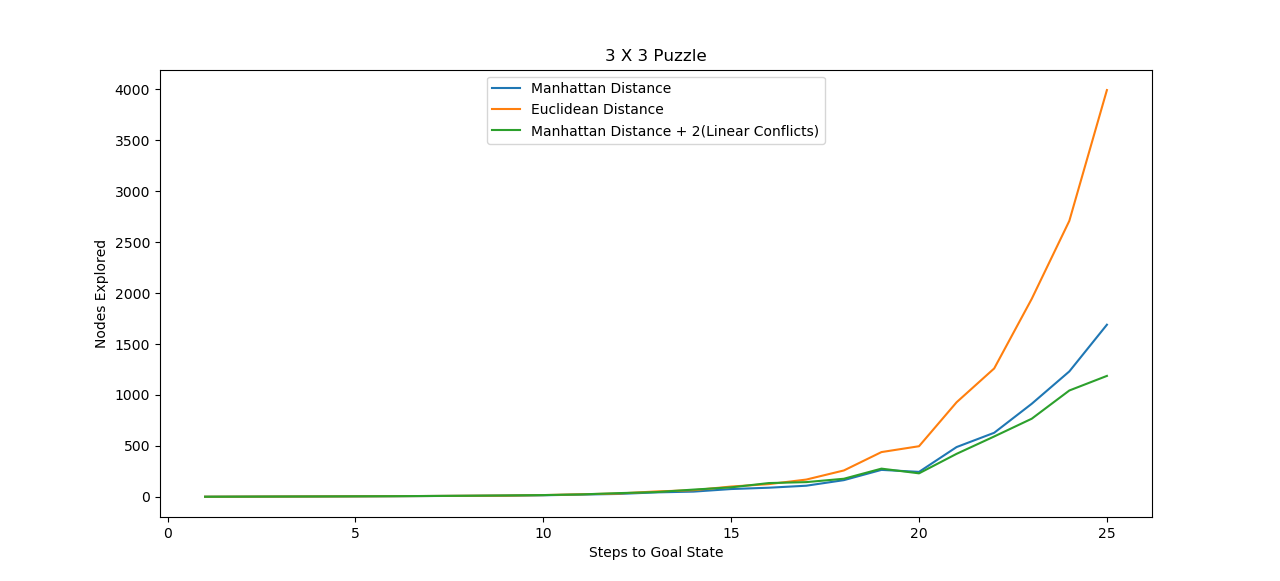
\includegraphics[width=\textwidth]{fig1.png}
    \caption{Performance of the three different heuristics under varying levels of k-puzzle difficulty.} \label{fig1}
    \end{figure}

In the analysis we will denote the Euclidean, Manhattan, and Manhattan + Linear Conflicts heuristics as E, M and L respectively. \\ 
For both the time and space complexity of the A star search using all 3 heuristics, we may observe that for lower values of steps required to reach the goal \( n \leq 15 \) is approximately the same. However, for higher step values, M and L outperforms E in terms of Time and Space complexity. This is in line with how the E will always be dominated by M and L, which explains the huge difference performance in time and space complexity. \\
Comparing the time and space complexity of the A star algorithm using M and L, we find that the time and space complexity is almost exactly identical for lower step values \( n \leq 22 \). However for values higher than that, we can observe that L outperforms M in terms of both time and space complexity. This is also in line with how L dominates M which translates directly into time and space efficiency \cite[p104]{stuart_russell_artifical_2010}. \\
Our group also calculated the actual time (in seconds) required to run the A star algorithm using all 3 heuristics.(where we put) It is interesting to note that while both M and L outperforms E, L actually takes longer time to solve the puzzle (in seconds) compared to when M is used. This is primarily because of the extra time required to calculate L for each node before it is put in the frontier. \\
In conclusion, our experiment has shown that more dominant heuristics prove to be more efficient in terms of time and space complexity. However, in terms of actual time taken, a better heuristic is not guaranteed to be faster (in this case of the usage of L being slower than M in real time) as it is ultimately dependent on the amount of actual time needed to compute the heuristic itself.

%
% ---- Bibliography ----
%
% BibTeX users should specify bibliography style 'splncs04'.
% References will then be sorted and formatted in the correct style.
%
\bibliographystyle{splncs04}
\bibliography{CS3243_project_1}

\begin{thebibliography}{8}
\bibitem{ref_article1}
Author, F.: Article title. Journal \textbf{2}(5), 99--110 (2016)

\bibitem{ref_lncs1}
Author, F., Author, S.: Title of a proceedings paper. In: Editor,
F., Editor, S. (eds.) CONFERENCE 2016, LNCS, vol. 9999, pp. 1--13.
Springer, Heidelberg (2016). \doi{10.10007/1234567890}

\bibitem{ref_book1}
Author, F., Author, S., Author, T.: Book title. 2nd edn. Publisher,
Location (1999)

\bibitem{ref_proc1}
Author, A.-B.: Contribution title. In: 9th International Proceedings
on Proceedings, pp. 1--2. Publisher, Location (2010)

\bibitem{ref_url1}
LNCS Homepage, \url{http://www.springer.com/lncs}. Last accessed 4
Oct 2017
\end{thebibliography}

\appendix
\section{Proof for Manhattan Distance Consistency}
\label{appendix:manhat_cons}

To prove that Manhattan Distance is consistent.
\begin{proof} Proof by Cases
    \begin{enumerate}
        \item \( |h(n') - h(n) = 1| \) (\( \because c(n, a, n') = 1 \), any node n' is 1 step away from node n)
        \item Case 1: \( h(n') = h(n) + 1 \)
        \begin{enumerate}
            \item \( h(n) \leq h(n) + 1 + 1 \implies h(n) \leq h(n') + c(n, a, n') \)
        \end{enumerate}
        \item Case 2: \( h(n') = h(n) - 1 \)
        \begin{enumerate}
            \item \( h(n) \leq h(n) - 1 + 1 \implies h(n) \leq h(n') + c(n, a, n') \)
        \end{enumerate}
        \item For both cases of \( h(n') \), \( h(n) \) is consistent. (\(\bullet\))
    \end{enumerate}
\end{proof}

\end{document}
